\documentclass[10pt]{article}
\usepackage{../../local}


\newcommand{\classcode}{Physics 112}
\newcommand{\classname}{Introduction to Statistical and Thermal Physics}
\renewcommand{\maketitle}{%
\hrule height4pt
\large{Eric Du \hfill \classcode}
\newline
\large{HW 02} \Large{\hfill \classname \hfill} \large{\today}
\hrule height4pt \vskip .7em
\normalsize
}
\linespread{1.1}
\begin{document}
	\maketitle
	\section*{Collaborators}
	I worked with \textbf{Andrew Binder}, and \textbf{Adarsh Iyer} to complete this homework.
	\section*{Schroeder 2.5 (5 pts)}
	For an Einstein solid with each of the following values of $N$ and $q$, list all of the possible 
	microstates, count them, and verify formula 2.9.
	\begin{enumerate}[label=\alph*)]
		\item $N = 3, q = 4$
			\addtocounter{enumi}{2}

			\begin{solution}
				Here we'll just generate a table and show out all the microstates, just like how it's 
				done in the book:
				\begin{center}
					\begin{tabular}{c|c|c|c}
						Oscillator & \#1 & \#2 & \#3\\
						\hline 
								   & 1 & 1 & 2\\
								   & 1 & 2 & 1\\
								   & 2 & 1 & 1\\
								   & 1 & 0 & 3\\
								   & 1 & 3 & 0\\
								   & 0 & 1 & 3\\
								   & 0 & 3 & 1\\
								   & 3 & 1 & 0\\
								   & 3 & 0 & 1\\
								   & 4 & 0 & 0\\
								   & 0 & 4 & 0\\
								   & 0 & 0 & 4\\
								   & 2 & 2 & 0\\
								   & 2 & 0 & 2\\
								   & 0 & 2 & 2
					\end{tabular}
				\end{center}
				In total there are 15 different configurations. Plugging it into the formula, we get:
				\[
					\Omega(3, 4) = {3 + 4 - 1 \choose 4} = {6 \choose 4} = 15
				\] 
				as desired.
			\end{solution}
		\item $N = 4, q = 2$

			\begin{solution}
				Just like the previous problem, we generate a table:
				\begin{center}
					\begin{tabular}{c|c|c|c|c}
						Oscillator & \#1 & \#2 & \#3 & \#4\\
						\hline
								   & 0 & 0 & 1 & 1\\
								   & 0 & 1 & 0 & 1\\
								   & 1 & 0 & 0 & 1\\
								   & 0 & 1 & 1 & 0\\
								   & 1 & 0 & 1 & 0\\
								   & 1 & 1 & 0 & 0\\
								   & 0 & 0 & 0 & 2\\
								   & 0 & 0 & 2 & 0\\
								   & 0 & 2 & 0 & 0\\
								   & 2 & 0 & 0 & 0
					\end{tabular}
				\end{center}
				So there are 10 possible configurations. Again, using formula 2.9:
				\[
					\Omega(4, 2) = {4 + 2 - 1 \choose 2} = {5 \choose 2} = 10
				\] 
				as desired.
			\end{solution}
			\addtocounter{enumi}{1}
		\item $N = 1, q = \text{anything}$

			\begin{solution}
				Since $N = 1$, then whatever $q$ is, all those units of energy must go into the single 
				particle that we have, so $\Omega = 1$ in this case. Using formula 2.9:
				\[
					\Omega(1, q) = {1 + q - 1 \choose q} = {q \choose q} = 1
				\] 
			\end{solution}
		\item $N = \text{anything}, q = 1$

			\begin{solution}
				Since we only have one energy packet and there are $N$ different particles, then there are 
				consequently $N$ different ways we can choose where to give this ``energy packet,'' hence 
				this gives us $\Omega = N$. 

				This is also confirmed by the formula 
				\[
					\Omega(N, 1) = {1 + N - 1 \choose 1} = {N \choose 1} = N
				\]
			\end{solution}
	\end{enumerate}

	\pagebreak
	\section*{Schroeder 2.8 (5 pts)}
	Consider a system of two Einstein solids, $A$ and $B$, each containing 10 oscillators, sharing a total 
	of 20 units of energy. Assume that the solids are weakly coupled, and that the total energy is 
	fixed. 
	\begin{enumerate}[label=\alph*)]
		\item How many different \textit{macro}states are available to this system?

			\begin{solution}
				The macrostate is defined as the amount of energy in $A$ and amount of energy in $B$. There 
				are 21 possible configurations, since the minimum amount of energy in one of the Einstein
				solids (which automatically determines the energy in the other) is 0 units, and the 
				maximum is 20 units.
			\end{solution}
		\item How many different \textit{micro}states are available to this system?

			\begin{solution}
				We use formula 2.9, where $N = 20$ and $q = 20$:
				\[
					\Omega(20, 20) = {39 \choose 20} = 6.89 \times 10^{10}	
				\] 
			\end{solution}
		\item Assuming that this system is in thermal equilibrium, what is the probability of finding all the 
			energy in solid $A$?

			\begin{solution}
				There is only one configuration in which all the energy is in solid $A$, so the probability 
				is $\frac{\Omega(10, 20)}{\Omega(\text{all})} = 1.45 \times 10^{-4}$.
			\end{solution}
		\item What is the probability of finding exactly half of the energy in solid $A$?

			\begin{solution}
				We need to calculate the number of microstates where exactly 10 units of energy are found within
				solid $A$ and also within solid $B$. This means that we can treat solids $A$ and $B$ as 
				independent, and multiply the two counts together. Then, we divide by the total 
				number of microstates to finally get our proability. Thus:
				\[
					\Omega(AB) = \frac{{19 \choose 10}{19 \choose 10}}{{39 \choose 10}} \approx 12\%
				\] 
			\end{solution}
		\item Under what circumstances would this system exhibit irreversible behavior?

			\begin{solution}
				This system would exhibit irreversible behavior whenever we let it move toward thermal 
				equilibrium, or in other words let the system settle into its most likely state. 
			\end{solution}
	\end{enumerate}

	\pagebreak

	\section*{Schroeder 2.18 (10 pts)}
	Use Stirling's approximation to show that the multiplicity of an Einstein solid, for any large values of $N$
	and $q$, is approximately
	\[
		\Omega(N, q) \approx \frac{\left( \frac{q + N}{q} \right)^q \left( \frac{q + N}{N} \right)^N}
		{\sqrt{2 \pi q(q + N) / N} }
	\] 
	The square root in the denominator is merely large, and can often by negelcted. However, it is needed 
	in Problem 2.22. (Hint: First show that $\Omega = \frac{N}{q + N}\frac{(q + N)!}{q! N!}$. Do not 
	neglect the $\sqrt{2\pi N} $ in Stirling's approximation.

	\begin{solution}
		First, we do the hint:
		\[
			\Omega(N, q) = {N + q - 1 \choose q} = \frac{(N + q - 1)!}{q!(N-1)!} = \frac{N}{N + q}
			\frac{(N + q)!}{q! N!}
		\] 
		Now, we apply Sterling's formula in the form $x! = x^xe^{-x}\sqrt{2\pi x}$:
		\begin{align*}
			\Omega(N, q) &\approx \frac{N}{N+q}\frac{(N + q)^{N + q} e^{-(N + q)} \sqrt{2 \pi (N + q)}}{q^q
			e^{-q} \sqrt{2 \pi q} \cdot N^N e^{-N} \sqrt{2 \pi N}} \\
						 &= \frac{N}{N + q} \frac{(N + q)^{N + q}}{N^N q^q} \cdot \sqrt{\frac{N + q}{2\pi Nq}} \\
						 &= \frac{\left( \frac{N + q}{N} \right)^N\left( \frac{N + q}{q} \right)^q}
						 {\sqrt{\frac{2 \pi Nq}{(N + q)} \cdot \frac{(N + q)^2}{N^2}}} \\
						 &= \frac{\left( \frac{N + q}{N} \right)^N\left( \frac{N + q}{N} \right)^q}
						 {\sqrt{2 \pi q(N + q) / N}}
		\end{align*}
		Sorry if I"m not showing \textit{every} single step of algebra, if I did then this simplification would
		take way too long.
	\end{solution}
	\pagebreak
	\section*{Ising Ferromagnet (15 pts)}

	Consider a system of $N$-magnetic moments each of which takes binary values $\sigma_i = \pm 1$ with 
	$i = 1, 2, \dots, N$. So there are $\Omega(\text{all}) = 2^N$ microstates, just like the 2-state model. 
	The energy, however, takes the form of a \textit{ferromagnet}

	\[
		E = -J \sum_{i = 1}^{N - 1} \sigma_i \sigma_{i + 1}
	\] 
	Note that the first and last spin talk only with the spin to their right/left respectively (the geometry is 
	a finite-length chain.)

	\begin{enumerate}[label=\alph*)]
		\item What are the very lowest energy microstates of the ferromagnet, and what are their energy? (We call
			these the ground states.) What do the microstates look like with an energy just above them?

			\begin{solution}
				To create the lowest energy state, we want $\sigma_i \sigma_{i + 1} = 1$, this can happen 
				in two different ways: either $\sigma_i = \sigma_{i + 1} = 1$ or $\sigma_i = \sigma_{i +1} = -1$.
				Therefore, the lowest energy microstate is one where all the magnetic moments are aligned 
				with one another. Here, since all $\sigma_i = \pm 1$, then this means that this state
				has an energy $E = -J(N - 1)$. Visually this is:
				\[
					\underbrace{\uparrow \cdots \uparrow \cdots \uparrow}_{N}
				\] 
				To generate the next energy, notice that when two consecutive $\sigma_i$ are equal, it actually 
				doesn't matter whether they're spin up or spin down - they contribute the same amount to 
				the final summation. Therefore, the only time we will increase the energy in the system when 
				we have the case where $\sigma_i = -\sigma_{i +1}$ or vice versa.

				Consider the case where there are ``domains of moments,'' where we have a chain of moments
				that are of all aligned with one another. This contributes the smallest amount of energy gain, 
				since it introduces only one pair of moments which are anti-aligned. Therefore, the 
				energy state just above them is the state where we have two domains of moments, or 
				alternatively one invisible ``wall'' between them. Visually, this looks like:
				\[
				\uparrow \dots \uparrow \vert \downarrow \cdots \downarrow
				\] 
				where the vertical line here denotes our ``wall'' where the spins flip. This contributes the 
				lowest energy gain, and hence it is the energy just above the ground state. 
			\end{solution}
		\item Derive an expression for the total number of microstates $\Omega(N, q)$ where $E = -J(N - 1) + 
			J 2q$. Hint: there is a clever trick you can apply here which maps the problem almost exactly to one 
			we solved in class!

			\begin{solution}
				We know that $E = -J(N - 1)$ is the ground state energy, so therefore we need to introduce 
				$2Jq$ energy into the system. Notice that when we introduce a wall, we add $2J$ units of 
				energy, since we change that particular product of $\sigma_i \sigma_{i+1}$ from $-J$ to 
				$J$. Therefore, 
				we require $q$ walls to generate $2Jq$ energy. 

				Effectively, this means our problem becomes finding the number of ways of distributing $q$ walls among $N$
				items, which is exactly the stars and bars problem. Therefore, the number of ways is:
				\[
					\Omega(N, q) = {N - 1 \choose q}
				\] 
				Finally, consider the fact that if we flip \textit{all} the spins, it doesn't change the 
				energy (since the summation doesn't prefer spin up over spin down), so for every configuration
				we count, there's a corresponding one with all the spins flipped. Therefore, the total 
				number actually is:
				\[
					\Omega(N, q) = 2{N  - 1 \choose q}
				\] 
			\end{solution}
	\end{enumerate}

	\pagebreak
	\section*{State Counting (20 pts)}
	I would like to conduct numerical experiments of the ideal gas, but it is a bit tricly because you have 
	to solve $F = ma$ for colliding particles. So, in the spirit of the ``spherical cow", in this problem you 
	will develop an approximate treatment of a gas by breaking up space into a discrete grid. 

	For simplicity, we will assume our particles move only in the 2D $x$-$y$ plane. We discretize space 
	into a square grid of small boxes each of volume $\Delta r^2$, labeled by their centers $(x, y)$. Now
	here is where we make a simplification: rather than keeping track of the \textit{exact} location of each 
	particle, we will only keep track of the number of particles in each box, $n(x, y) = 0, 1, 2, \dots$. 
	The microstate of the system is then labeled by the collection of integers $\{n(x, y)\}$ where 
	$\sum_{x,y} n(x, y) = N$ is the total number of particles. 
	\begin{enumerate}[label=\alph*)]
		\item Explain why $\{n(x, y)\}$ is sufficient to recover the precise location of all the particles if we 
			take $\Delta r^2 \to 0$ while holding the average partilce density fixed. (You may wonder about 
			permutations of the particles \ldots we'll come back to this when we discuss the Gibbs Paradox)

			\begin{solution}
				Consider the case where we have a particle in our particular grid. Our uncertainty 
				in the position of that particle comes directly from the size of the square,  
				since we can't say anything about where inside the square the particle resides. Therefore, 
				if we reduce the size of the square (i.e. $\Delta r \to 0$), then we are reducing 
				our uncertainty in the location of all particles, meaning that by just shrinking $\Delta r$ 
				it is indeed sufficient to recover the precise location.
			\end{solution}
	\end{enumerate}
	Henceforth, we'll choose units such that $\Delta r^2 = 1$ for notational simplicity. There are $V = L_x \cdot
	L_y$ such boxes labeled by integers pairs $(x, y)$. 
	\begin{enumerate}[label=\alph*), resume]
		\item Suppose the energy is entirely independent of $\{n(x, y)\}$, is an ideal gas without a 
			gravitational potential. How many microstates $\Omega(V, N)$ are there for a system with $V$-boxes
			and $N$ particles? Hint: you already know the answer!

			\begin{solution}
				There's $N$ particles that we have to place into $V$ boxes, this is the same problem 
				as having $N$ units of energy, and we need to place it into $V$ oscillators. Therefore, 
				the number of microstates is: 
				\[
					\Omega(V, N) = {V + N - 1 \choose N} 
				\] 
			\end{solution}
		\item Consider an $V = L_x \times L_y = 20 \times 20$ system which we partition into $V_A = 9 \times 
			20$ region and a $V_B = 11 \times 20$ region, with $N = N_A + N_B = 100$ particles. Following the 
			fundamental assmption of statistical mechanics (and assuming particles are never created or 
			destroyed), obtain a mathematical expression for the probability $P(N_A)$ to 
			observe $N_A$ particles in region $A$. Evaluate $P(N_A = 40)$ using e.g. Mathematica.

			\begin{solution}
				First note that we have the following expression for $P(N_A)$:
				\[
					P(N_A) = \frac{\Omega(V_A, N_A) \Omega(V_B, N_B)}{\Omega(\text{all})}
				\]
				We have 100 particles and $V = 400$, so $\Omega(\text{all}) = \Omega(400, 100)$. Then, 
				the volume of region $A$ is $V_A = 180$, $V_B = 220$, Therefore, we have:
				\[
					P(N_A) = \frac{{V_A + N_A - 1 \choose N_A} {V_B + N_B - 1 \choose N_B}}{{V + N - 1 \choose 
					N}} = \frac{{180 + 40 - 1 \choose 40}{220 + 60 - 1 \choose 60}}{{400 + 100 - 1 \choose 
					100}} \approx 0.048
				\] 
			\end{solution}
		\item Use Stirling's approximation in the form $\ln x! = x \ln x - x$ to approximately 
			bring $P(\mean{N_A})$ to the form $P(N_A) = P(N_A)e^{-\frac{1}{2}(N_A - \mean{N_A})^2 / \sigma^2}$.
			What is the average $\mean{N_A}$ and standard deviation $\sigma = \sqrt{\mean{(N_A - \mean{N_A})^2}}$
			for the parameters of Part 2? Hint: your answer will take a fairly nice form if expressed in 
			terms of $V$, $\frac{V_A}{V_B}, n = \frac{N}{V}, n_A = \frac{N_A}{V_A}$. If you'd like to use 
			Mathematica at some point that's fine (I did): just be explicit in what step it was used for. 

			\begin{solution}
				So this problem was incredibly annoying, myself and a couple friends spent a very long time 
				and basically got nowhere with the expression. We first simplified the expression 
				using Stirling's formula by hand, and we got the following equations:
				\begin{align*}
					\ln\Omega(V_A, N_A) &= \ln \Omega(V_A, \mean{N_A}) + \epsilon \mean{N_A} \ln \left( \frac{\mean{N_A} + V_A}{\mean{N_A}} \right) \\
					\ln \Omega(V_B, N_B) &= \ln \Omega(V_B, N - \mean{N_A}) - \epsilon M \ln
					\left( \frac{N - \mean{N_A} + V_B}{N-\mean{N_A}} \right) \\
					\ln \Omega(V, N) &= (N + V)\ln(1 + n) - N \log n
				\end{align*}
				where we've defined $\epsilon = \frac{x}{\mean{N_A}}$, $x = N_A - \mean{N_A}$ and 
				$n = \frac{N}{V}$. Below are the photos of my work:
				\begin{center}
					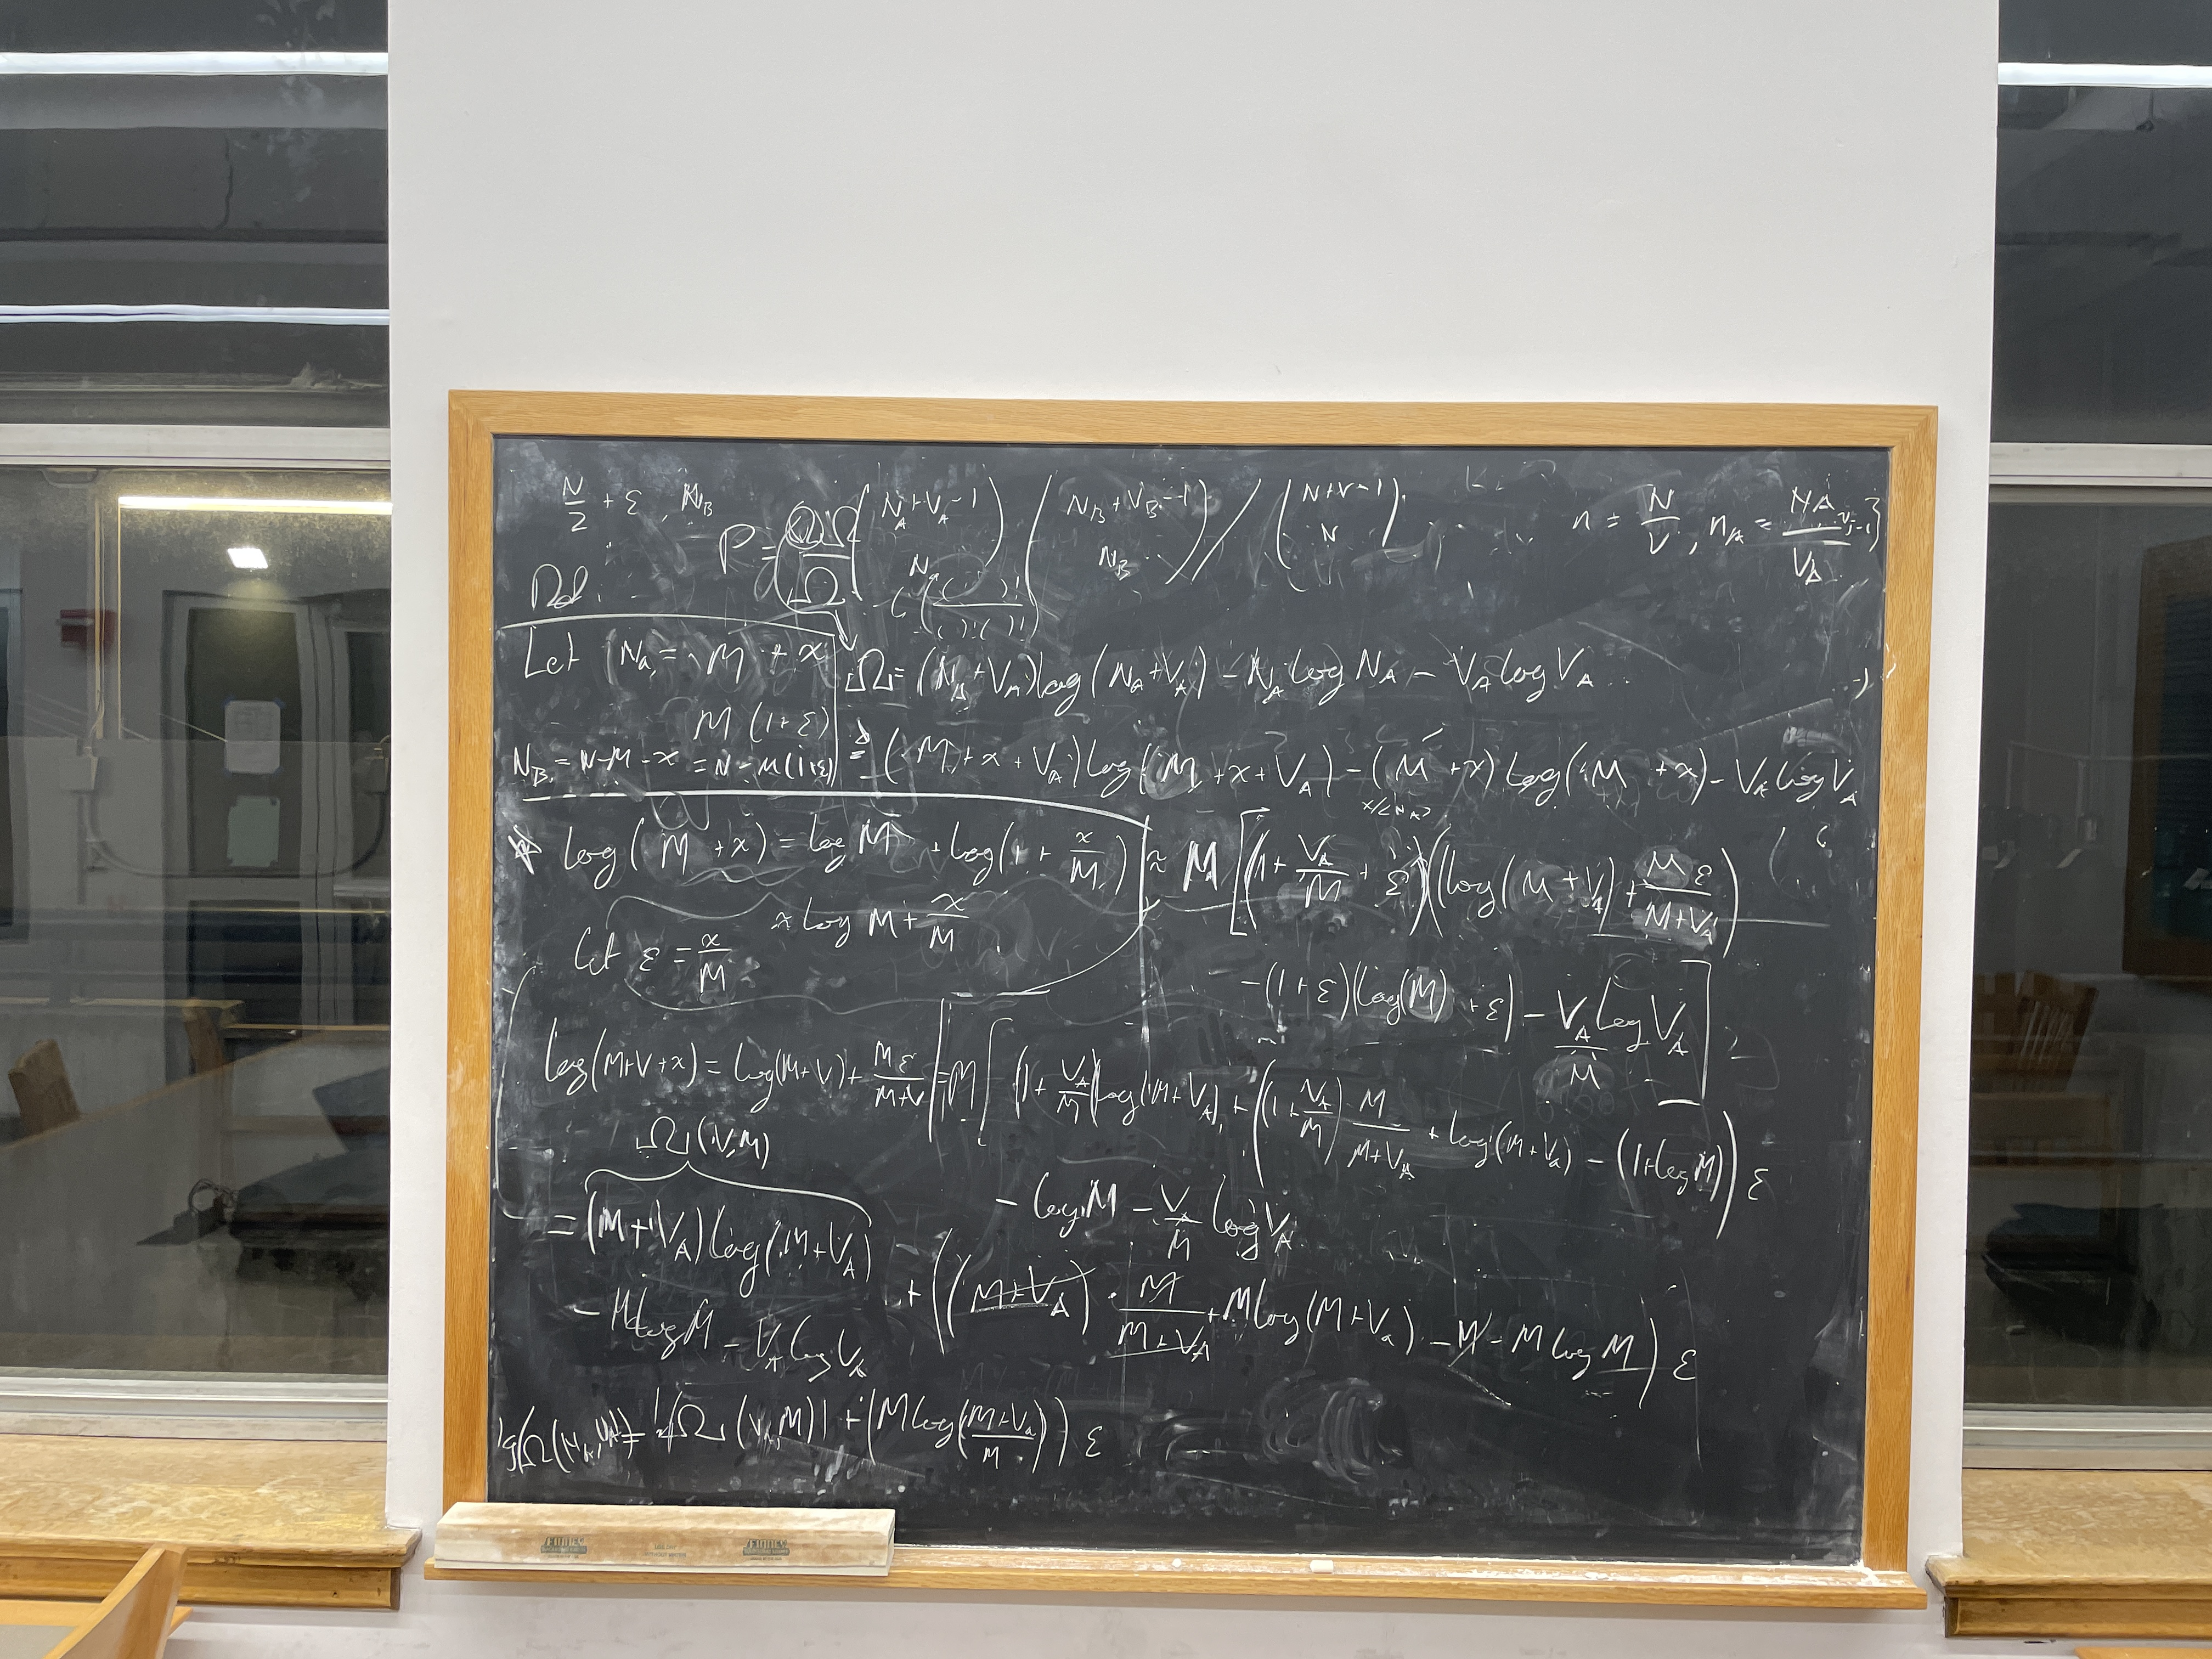
\includegraphics[scale=0.4]{bb1.jpg}
					\smallskip
					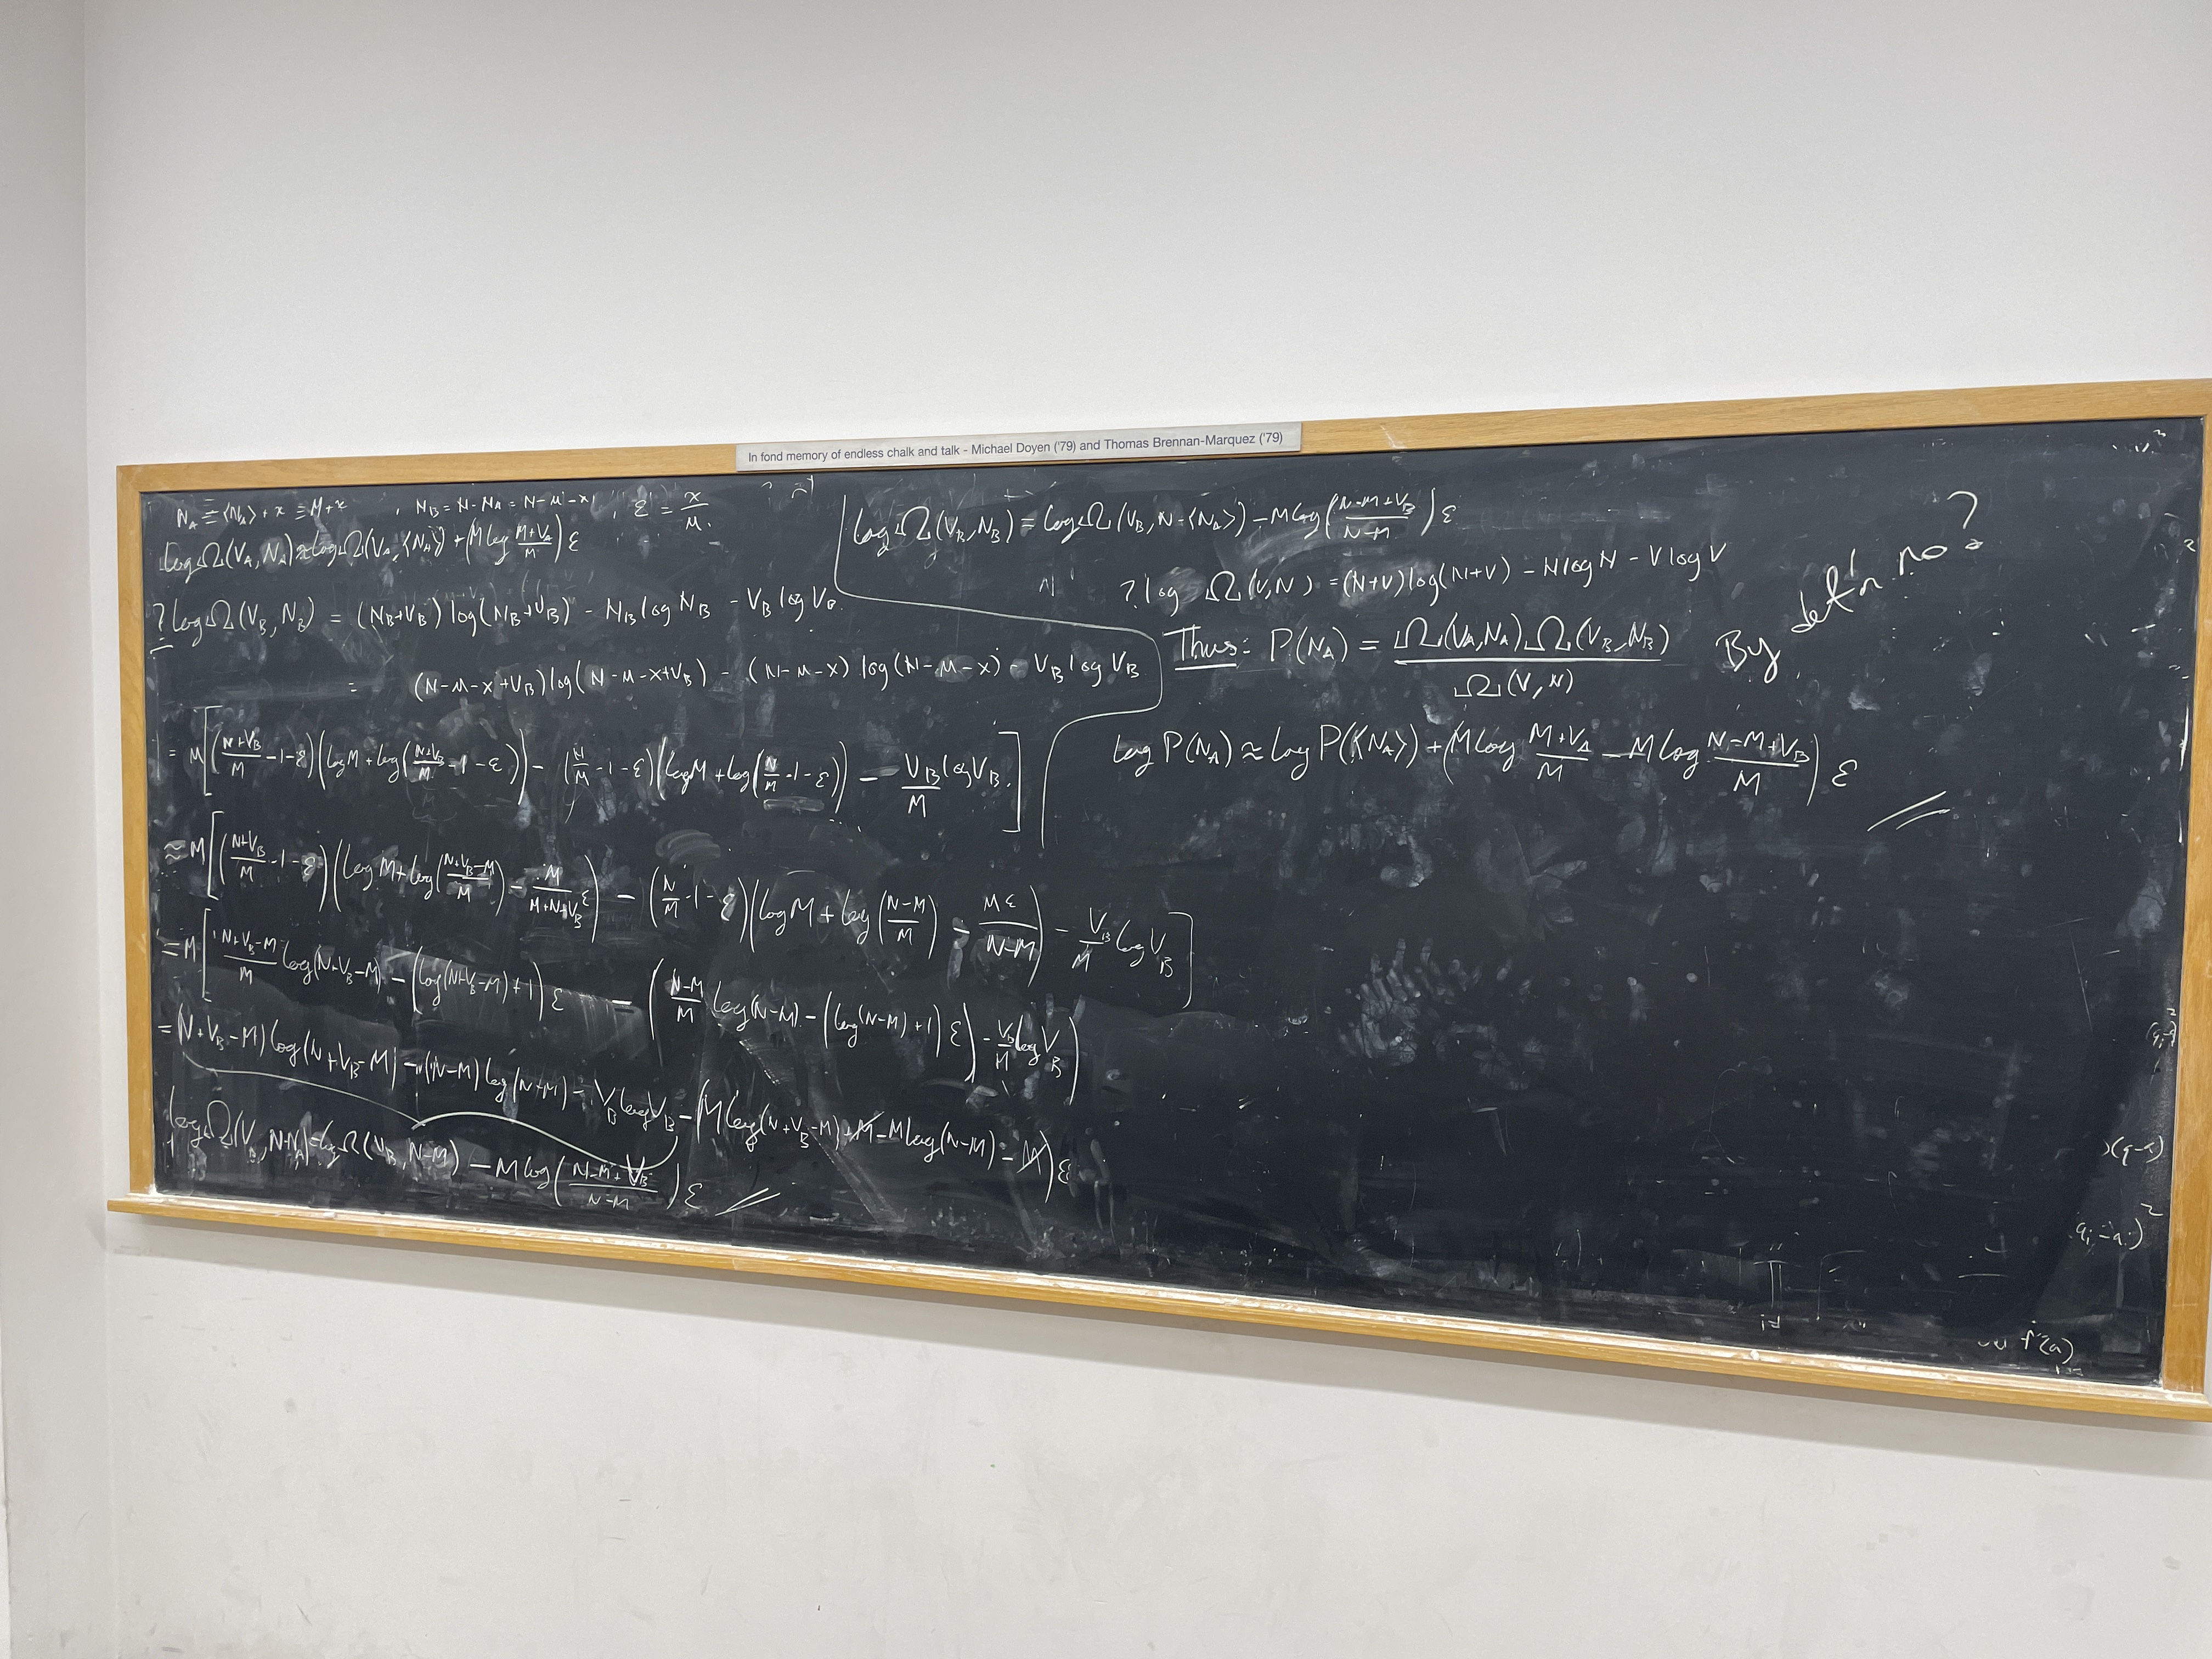
\includegraphics[scale=0.4]{bb2.jpg}
					\smallskip
					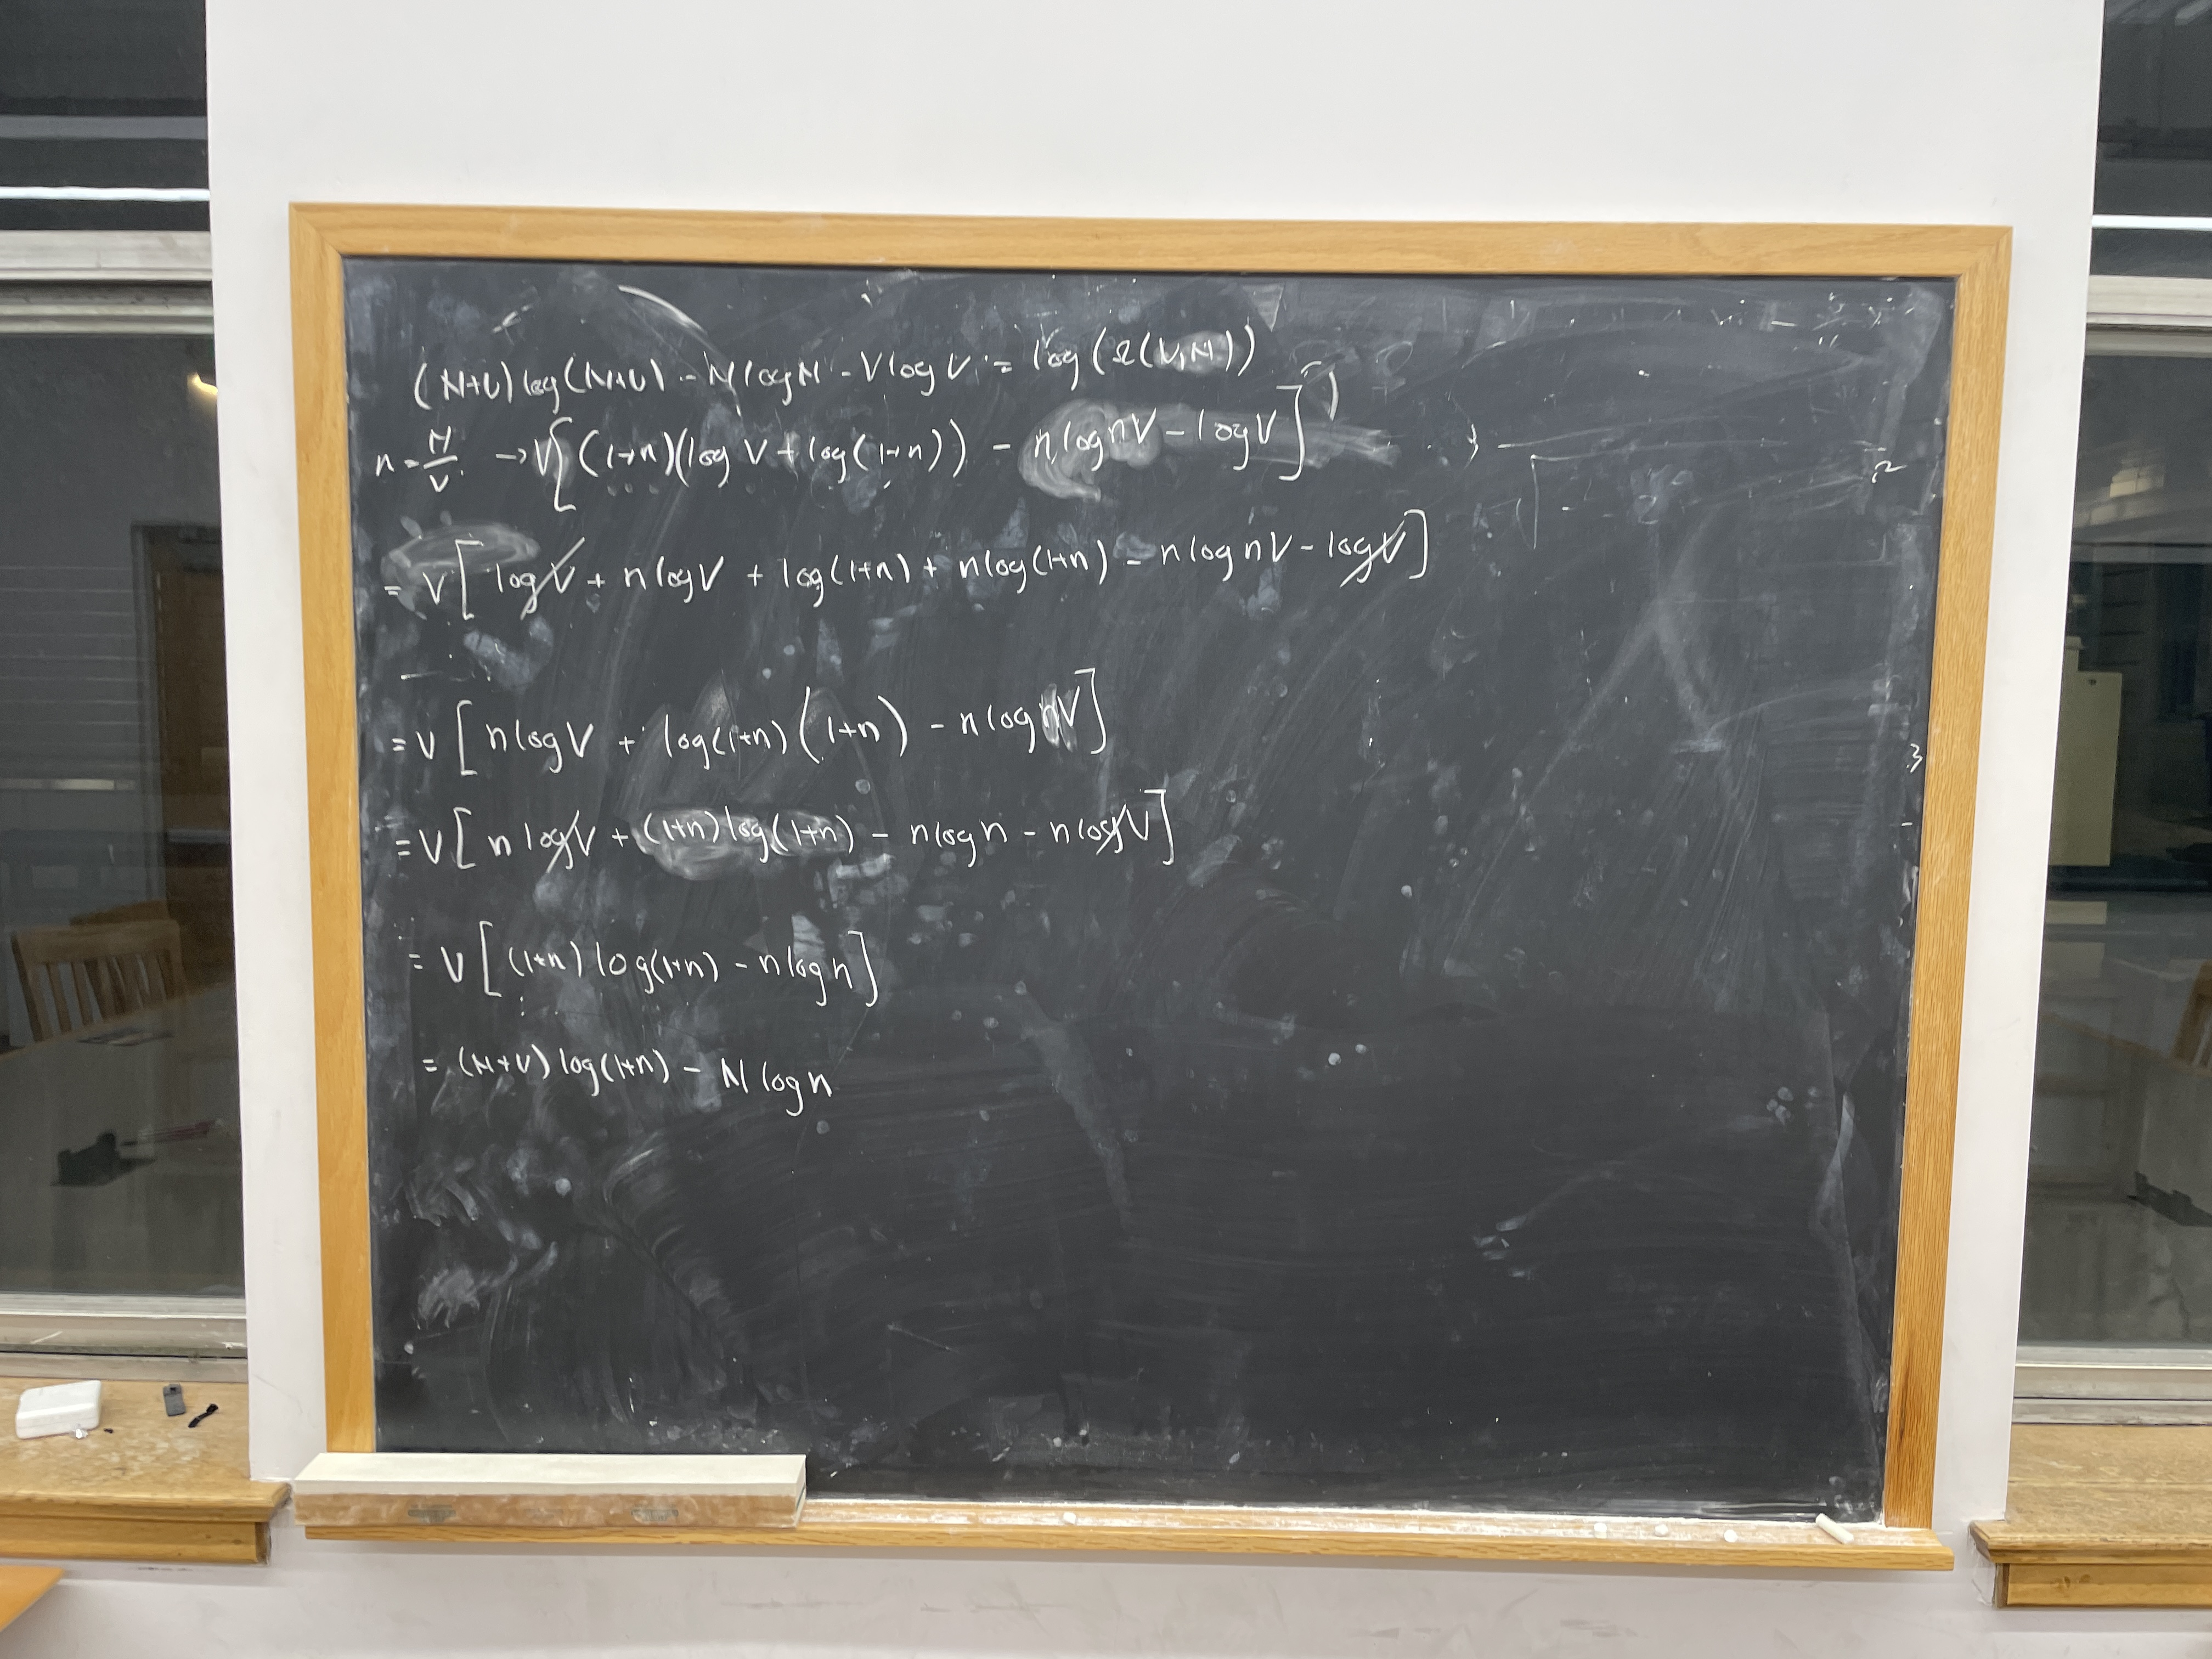
\includegraphics[scale=0.4]{bb3.jpg}
				\end{center}
				I didn't want to type out all the algebra since it would be a lot, but in essence, we expanded $N_A = \mean{N_A} + x$
				where $x$ is some small quantity, then performed the Taylor expansion of $\ln(1 + x)$ around 
				$x = 0$ wherever possible. We also used the suggested expressions of $n = \frac{N}{V}$ and $n_A = \frac{N_A}{V_A}$. We then simplified this further by using the initial expression for 
				$\Omega(V, N)$, but this ultimately didn't get us down to the desired form.
			\end{solution}
		\item We have approximated the gas' microstates by $\{n(x, y)\}$. As $\Delta r^2 \to 0$, do you think
			this gives a reasonable counting of all the microstates of a mono-atomic ideal gas? Or are we 
			missing degrees of freedom? Explain.

			\begin{solution}
				This does not give a reasonable counting, since $\{n(x, y)\}$ only gives information about 
				the \textit{position} of the particles, but not its momentum. Since we're
				missing these degrees of freedom in our calculations, this is not an accurate 
				counting of all the microstates. 
			\end{solution}
	\end{enumerate}

	\pagebreak
	\section*{Problem 6: Numerical Simulation (20 pts)}
	
	I couldn't find a good way to attach the file, so I downloaded my python code by converting it to a PDF
	and attached it below. However, due to the way that the code blocks render, the formula doesn't wrap, but 
	instead just goes off the page, so for some lines only half of the code in that line is visible. 
	Unfortunately there isn't an easy fix for this, but if there's a way please do let me know so I can do it 
	for future submissions.
\end{document}
